\documentclass[preprint,10pt]{sigplanconf}

% The following \documentclass options may be useful:
%
% 10pt          To set in 10-point type instead of 9-point.
% 11pt          To set in 11-point type instead of 9-point.
% authoryear    To obtain author/year citation style instead of numeric.

\usepackage{amsmath}
\usepackage{listings}
\usepackage{graphicx}
\usepackage{color}
\usepackage{float}
\usepackage{subfig}
\usepackage{multirow}

\newcounter{copyrightbox}

\newcommand{\monospace}[1]{\texttt{\small #1}}

\newcommand{\ry}[1]{\textcolor{red}{[RY: #1]}}

\lstset{
  captionpos=t,
  tabsize=2,
  numbers=left,
  numberstyle=\tiny,
  numbersep=5pt,
  breaklines=true,
  showstringspaces=true,
  basicstyle=\footnotesize\ttfamily,
  frame=none,
  emph={label},
  escapeinside={(*}{*)}
}

\begin{document}

\conferenceinfo{APPLC '12}{June 14, 2012, Beijing, China.} 
\copyrightyear{2012} 
\copyrightdata{[to be supplied]} 

%\titlebanner{banner above paper title}        % These are ignored unless
%\preprintfooter{short description of paper}   % 'preprint' option specified.

\title{A Runtime System for Generalized Committed Choice}
%\subtitle{Subtitle Text, if any}

\authorinfo
{Xiao Jia \hspace*{1cm} Kenny Q. Zhu}
{Shanghai Jiao Tong University}
{\{xjia,kzhu\}@cs.sjtu.edu.cn}

\authorinfo
{Joxan Jaffar \hspace*{1cm} Roland H.C. Yap}
{National University of Singapore}
{\{joxan,ryap\}@comp.nus.edu.sg}
%\authorinfo{Name2\and Name3}
%           {Affiliation2/3}
%           {Email2/3}

\maketitle

\begin{abstract}
Traditional nondeterministic programming constructs 
  (Dijkstra guards,
% \cite{Dijkstra:discipline}, 
CCP \cite{Saraswat:CCP} 
  and deep guards \cite{Smolka94:OzCalculus}) 
  do not allow operations which modify the runtime environment 
  without committing to a particular alternative. 
Generalized committed choice (GCC) 
  allows speculative computations across different alternatives 
  to execute in parallel and isolation. 
Speculation implicitly forks 
  an environment into separate ones for the alternatives and 
  later one of these environments can be committed to \cite{JaffarYZ07}. 
Speculations from concurrent processes can nevertheless interleave and 
  synchronize against each other. 
In this paper, we present a concrete architecture, 
  its implementation and optimizations for GCC where the store of 
  the environment is in the form of record spaces. 
Our prototype implementation allows GCC to be embedded in traditional 
  languages such as C/C++. 
Preliminary experimental results show that our runtime and GCC extension 
  is a suitable coordination language for programming multiple 
  distributed agents which employ speculation and choices. 
\end{abstract}

% Dont think we need this for the submission - gain some space
% \category{D.3.3}{Programming Languages}
%                 {Language Constructs and Features}
% %               [Concurrent programming structures]
% 
% \terms
% Languages, Design, Performance
% 
% \keywords
% Coordination languages, Generalized committed choice, Runtime system

\section{Introduction}  % Section 1

% What is the problem area you are working in?
% Why is it important?
% Why is the problem of interest and importance to the larger community?
%A complete programming model can be built out of two separate pieces -- 
%  the computation model, which allows programmers to build a single 
%  computational activity, and 
%  the coordination model, which is the glue that binds separate activities into an ensemble \cite{GelernterC92}. 
A coordination language embodies a coordination model and is responsible for 
  the creation of, and the support of communication among, computational activities. 
%Computation itself is incomplete and useless without coordination. 
%Classical computation languages have some flavors of 
%  simple coordination of computations in order to make itself useful. 
%However, coordination models and languages are not yet investigated much. 
%We believe that coordination improvements are of great significance and 
%  will contribute to a more complete and powerful programming model. 
% What is the specific problem considered in this paper?
The generalized committed choice (GCC) is a coordination model of 
a don't-know nondeterminism choice construct 
which allows the commit to occur anywhere within the choice \cite{JaffarYZ07} 
and strives for maximal inter-play of choices between agents
to achieve beneficial speculation. GCC was proposed as a coordination model 
for speculation among concurrent agents.
% What are the main contributions of your paper? (IMPORTANT)
In this short paper, we report our preliminary progress in developing 
a concrete GCC runtime system. This work has the following contributions: 

\begin{itemize}
  \item We demonstrate GCC as a usable and practical coordination model for 
          traditional programming languages such as C/C++ by 
          embedding GCC constructs in regular C/C++ programs and by 
          employing record stores as the data model; 
  \item We extend the multi-world concept \cite{JaffarYZ07} 
          to the notion of \emph{multiple universe} 
          which is transparent to programmers and 
          crucial to handling the exponential explosion of multiple worlds; 
  \item We show the viability of our system by two non-trivial examples
          and their runtime statistics.
\end{itemize}

The remainder of this paper is structured as follows. 
The rest of this section gives an overview of the GCC model and 
introduces the usage in concrete actual agent programs. 
Section 2 presents the overall system architecture. 
Section 3 discusses several optimization considerations. 
Section 4 gives some preliminary experimental results which
show that speculative computation with GCC agents is practical.
%Section 5 concludes this paper. 

\subsection{Motivation}

We use the motivating example for GCC \cite{JaffarYZ07}. 
Bob and Jill participate in an online trading system. 
Bob wants to upgrade his camera and Jill wants to downgrade. 
Their preferences which are exclusive
(denoted by \monospace{XOR}) are:

Bob's agent: (sequencing is denoted by `;')
{\small \vspace{-2mm}
\begin{verbatim}
    (buy(goodlens); sell(averagelens)) XOR
    (buy(goodcam); sell(averagecam))
\end{verbatim}
\vspace{-1mm}}

Jill's agent:
{\small \vspace{-2mm}
\begin{verbatim}
    (sell(goodlens); buy(averagecam)) XOR
    (sell(goodcam); buy(averagecam))
\end{verbatim}
\vspace{-1mm}}

\monospace{Buy} and \monospace{sell} are synchronous actions which block
until there is a matching transaction.
Bob and Jill are not aware of each other, i.e. each agent acts independently. 
The objective is to satisfy as many agents as possible. 
In this example, GCC does this by creating four separate and 
isolated worlds arising from the potential interaction between
the combination of Bob and Jill's choices as the agent computation proceeds. 
Figure \ref{fig:multi-worlds} shows the effect of multiple worlds 
where {\tt lens()} denotes buying(selling) lens by Bob(Jill),
and {\tt cam()} denotes buying(selling) camera by Bob(Jill).
In this example, only in world $w_4$ can both agents be satisfied.\footnote{
$w_1$ cannot complete after the lens transaction while $w_2$ and
$w_3$ block.
}
This requires speculation where agents can continue to interact. 
The runtime system in this paper provides essential facilities  
  for embedding and implementing this example in 
  conventional languages such as C/C++. 

\begin{figure}
\begin{center}
    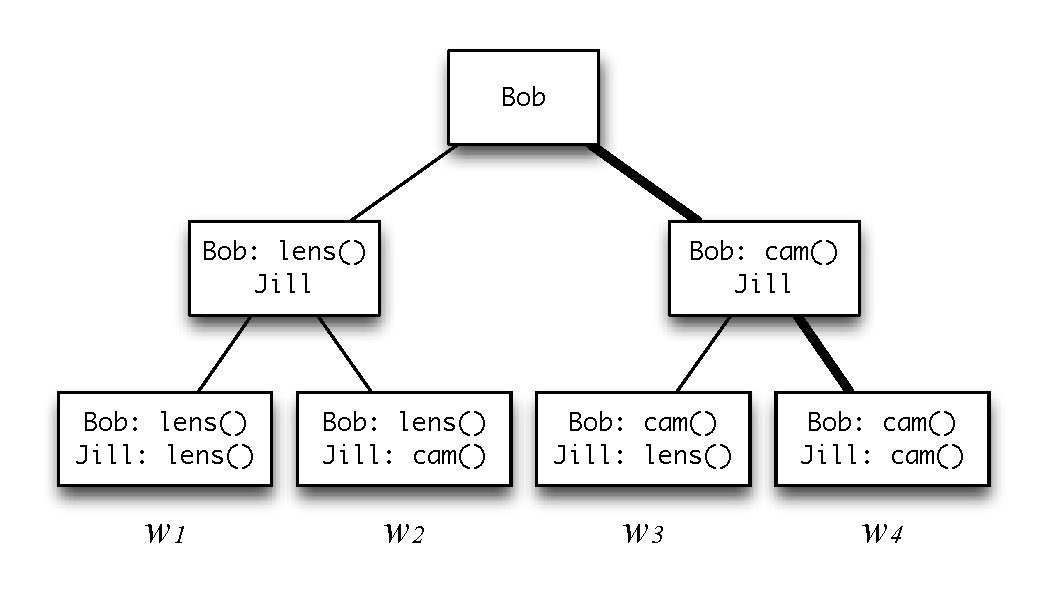
\includegraphics[width=0.4\textwidth]{eps/multi-worlds}
    \vspace{-3mm}
    \caption{The multiple worlds in Bob-Jill example}
    \label{fig:multi-worlds}
\end{center}
\end{figure}

\subsection{C Implementation of Bob-Jill Example}

We show the above example in the APIs in our runtime system --
the agents are \monospace{bob.cc} and \monospace{jill.cc}. 
Note that although the agents employ speculation and concurrency
  using GCC semantics, the embedding allows the agents to be written in
  vanilla-looking C (see Listing \ref{bob-cc} and \ref{jill-cc}) using
the following GCC coordination constructs in the runtime system:
\begin{center}
\begin{tabular}{c|l}
  \hline
  \monospace{gcc} & fork multiple choices \\
  \monospace{cm}  & commit me (commit to this choice) \\
  \monospace{cu}  & commit you (kill this choice) \\
  \hline
  \monospace{in}  & reads and removes a record from a record space \\
  \monospace{rd}  & non-destructively reads a record space \\
  \monospace{out} & produces a record, writing it into a record space \\
  \hline
\end{tabular}
\end{center}


\begin{lstlisting}[label=bob-cc,caption=\monospace{bob.cc}]
void lens()
  { buy(GoodLens); sell(AvgLens); cm(); }
void cam()
  { buy(GoodCam); sell(AvgCam); cm(); }
int main()
  { gcc(lens, cam); return 0; }
\end{lstlisting}

\begin{lstlisting}[label=jill-cc,caption=\monospace{jill.cc}]
void lens()
  { sell(GoodLens); buy(AvgCam); cm(); }
void cam()
  { sell(GoodCam); buy(AvgCam); cm(); }
int main()
  { gcc(lens, cam); return 0; }
\end{lstlisting}

\begin{lstlisting}[label=common-cc,caption=Common routines for trading]
enum Product
    { GoodLens, AvgLens, GoodCam, AvgCam };
enum Type { Ack, Buy, Sell };
struct Offer { Type s; Product p; int i; };
void parse(struct Offer *, char *) { /*...*/ }
void sell(Product p)
{ int id = generate_unique_id();
  out("s=%d,p=%d,i=%d", Sell, p, id);(*\label{line:out-sell}*)
  in("s=%d & i=%d & p?=1", Buy, id);(*\label{line:in-buy}*)
  out("s=%d,p=%d,i=%d", Ack, p, id);    }(*\label{line:out-ack}*)
void buy(Product p)
{ struct Offer f;
  parse(&f,
    in("s=%d & p=%d & i?=1", Sell, p));(*\label{line:in-sell}*)
  out("s=%d,p=%d,i=%d", Buy, p, f.i);(*\label{line:out-buy}*)
  rd("s=%d & i=%d & p?=1", Ack, f.i);   }(*\label{line:rd-ack}*)
\end{lstlisting}

Common trading routines are in Listing \ref{common-cc}. 
A trading transaction is a record of three elements: 
the trade type $s$, which can be {\tt Ack}, {\tt Buy}, or {\tt Sell}; 
the product type $p$, which can be {\tt GoodLens}, {\tt AvgLens}, 
{\tt GoodCam}, or {\tt AvgCam}; and the transaction number $i$, 
which is generated and guaranteed to be unique. 
When an agent wants to sell some product $p^*$, 
he produces a record {\tt (s=Sell, p=$p^*$, i=id)} (line \ref{line:out-sell}), 
where $id$ is a transaction number. 
Then he waits for someone to buy $p^*$ by 
{\tt in(s=Buy \& i=id \& p?=1)} (line \ref{line:in-buy}). 
When an agent wants to buy some product $p^*$, 
he consumes a record by {\tt in(s=Sell \& p=$p^*$ \& i?=1)} 
first (line \ref{line:in-sell}), 
and then {\tt out(s=Buy, p=$p^*$, i=id)} (line \ref{line:out-buy}). 
At the end of a transaction, 
the seller produces an {\tt Ack} record (line \ref{line:out-ack}) and 
the buyer reads it for acknowledgement (line \ref{line:rd-ack}). 

%The \monospace{in} function provided by our runtime system returns 
%  the string representation of a record. 
%\ry{maybe simplify by removing parse}
%The \monospace{parse} function in Listing \ref{common-cc} parses 
%  such a string representation and fills values into an \monospace{Offer}. 

\subsection{Related Work}

Earlier work \cite{JaffarYZ07} lays the theoretical foundation for GCC
  without addressing the practical details of employing GCC
  in conventional programming languages as well as a  
  practical data model for real-world applications. 
Our runtime system uses a data model for GCC
  called \emph{record space}, which uses Linda style tuples
  \cite{Gelernter85:Linda} with labels for tuple elements. 

Logic programming languages, e.g. Prolog, 
  search the solution space in a depth-first fashion. 
Shared Prolog \cite{BrogiC91} programs are composed of a set of parallel agents 
  that are Prolog programs extended by a guard mechanism. 
Coordination of the agents is controlled by programmers via a centralized 
  data structure roughly resembling a blackboard system \cite{Nii:Blackboard}. 

Deep guards \cite{Smolka94:OzCalculus,SchulteS94} in Oz \cite{Smolka94,SchulteSW94} 
  and its implementations, such as LVM \cite{Mehl:diss}, only enable 
  local computation spaces with monotonic constraint stores and 
  short-lived actors.
All local effects only become globally visible at the time of commit.
Such restrictions make it useless in the context of the applications
considered here such as real-time marketplaces with long transactions. 

\section{System Architecture} % Section 2

\begin{figure}
  \centering
  \subfloat[Physical deployment view]{
    \label{fig:deploy_view}
    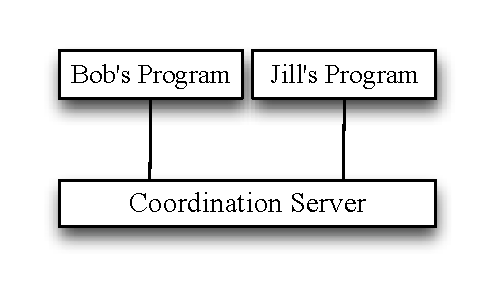
\includegraphics[width=0.26\textwidth]{eps/deploy-view}}
  \subfloat[Logical runtime view]{
    \label{fig:logical_view}
    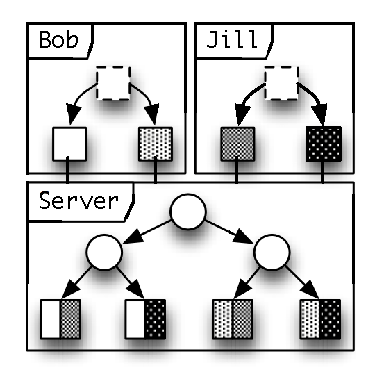
\includegraphics[width=0.18\textwidth]{eps/logical-view}} \\
  \caption{Logical runtime view}
\end{figure}

Agents can be distributed and
communicate through the \emph{coordination server} 
as shown in Fig. \ref{fig:deploy_view}. 
(Our prototype uses agents in Unix).
Two agents are initially two Unix processes which can
fork into multiple processes if they involve choices. 

Fig. \ref{fig:logical_view} depicts the logical view of runtime environment. 
Bob's program starts from a single process and then forks into two processes 
for the two choices (to buy good lens or good camera). 
Jill's program works similarly. 
The coordination server maintains all runtime information, such as 
the structure of all the worlds and the relationships among them. 
Each process in the agent's environment conceptually lives in 
one or more worlds. 
Processes from different agents live in the same world if they interact. 
There is a communication channel between each process and the server. 

%Fig. \ref{fig:multi-worlds} is a particular runtime view of the Bob-Jill example. 
%Assume that Bob's program gets executed first. The two agent programs will eventually 
%split into four isolated worlds. 

\section{Implementation and Optimizations} % Section 3

The main technical challenge in the implementation of GCC system is
  to contain the exponential growth of worlds because each world consumes
  valuable system resources. 
See  \cite{JaffarYZ07} for more details on the conceptual semantics of GCC.
In this section, we will present one key 
  implementation idea that tackle the challenge and then briefly discuss several
  other optimizations.

\subsection{Multiple Universe}
A \emph{universe} is a rooted tree of worlds along with their records. 
The records in a universe form a logical \emph{partition} of the 
  record space by record types. 
Agents that operate on different record types live in 
  different universes. Worlds only get multiplied if two agents with
  choices are interested in the same type of records. 

%{\bf KZ: It might be better to include a diagram to show the flow of
%evolution of the universes, the following text essentially talks 
%about this diagram.} 

At startup, an agent program lives outside any universe. 
Once the agent wants to operate on some type of records, 
it either migrates to the universe 
which owns that record type, or creates a new universe with that type. 
Let $U$ be a universe, $S(U)$ be the set of record types owned by 
the universe $U$. Suppose there are in total $n$ universes, 
$U_1,U_2,\dots,U_n$, in the runtime environment. 
When an agent program $P$ in universe $U_i (1\leq i\leq n)$ 
is about to operate on some record type $T$ 
(by \monospace{in}/\monospace{rd}/\monospace{out}), 
there are three cases: 
%\ry{not clear, the cases seem not disjoint?}
  \begin{itemize}
    \item $T \in S(U_i)$, then $P$ operates on $U_i$ as normal; 
    \item $\exists 1\leq j\leq n, j\neq i$, such that $T \in S(U_j)$, then 
          $U_i$ and $U_j$ are removed and replaced by $U_k=J(U_i,U_j)$ where 
          $J$ joins two universes together to form another tree of worlds. 
          $U_k$ is then added to the runtime environment for $P$ to operate on; 
    \item $\forall 1\leq j\leq n, T \not\in S(U_j)$, then 
          $S(U_i) \leftarrow S(U_i) \cup \{T\}$ and $P$ operates on $U_i$. 
  \end{itemize}

The type of a record is the set of labels of the elements in the record. 
For example, the record {\tt (a=1, b=2)} has the type $\{a, b\}$. 
Querying a record with constraints uses the label types,
e.g. querying 
only on $a$, the condition becomes {\tt ($p$ \& b?=1)} 
for {\tt in/rd} operations, where $p$ is a condition on $a$. 
The question mark $?$ is the \emph{existence operator} which 
evaluates to $1$ if the label exists, or $0$ otherwise. 

\subsection{Other Optimizations}

\begin{description}
  \item[Lazy forking] 
        allows \emph{asynchronous coordination} among 
        agent programs and the server, and implies a \emph{fork-on-need} mechanism. 
      For example, program $P$ starts with world $w$, 
        which is later split into two worlds, $x$ and $y$, by another program $Q$, 
        which has to fork, but $P$ doesn't need to, until it interacts with $w$.

  \item[Opportunistic forking] is introduced that when there are too many 
        \monospace{gcc()} requests at the same time, some of them will be 
        delayed randomly in order to limit the number of worlds. 

  \item[Condition triggering], 
        which is enabled by \emph{indexing} of record labels, 
        is available for record consuming and reading actions (\monospace{in} and \monospace{rd}). 
	Options for \monospace{in} and \monospace{rd} operations are:
	non-blocking, time-out and block until a condition.
%        which will return immediately, wait for a timeout, or block forever, for a condition. 

  \item[Storage sharing] works as a storage hierarchy where records are stored 
        as closer to the root as possible. New records are always written to 
        the current world. Searching a record starts from the current world, 
        and if not found, the searching continues in the parent world, etc. 
\end{description}

\section{Evaluation}  % Section 4

We evaluate our runtime system by running two examples 
which exemplify speculative computation inside choices.
The experiments ran on Linux on a
  4-core 2.0GHz Intel Xeon CPU with 8GB RAM. 
\begin{description}
  \item[Bob-Jill example]: 
	10 instances each of Bob and Jill agents;
%        10 instances of Bob's agent (Listing \ref{bob-cc}) along with 
%        10 instances of Jill's agent (Listing \ref{jill-cc}); 
  \item[Flight reservation example]: 
	10 instances of selling agents (Listing \ref{seller-cc}) and
        20 instances of buying agents (Listing \ref{buyer-cc}). 
\end{description}

We propose the flight reservation example as a potential application of GCC. 
Here flight agents sell tickets whenever they are available, and 
travelers are ticket buyers waiting for desired tickets. 
Travelers may want to buy a multi-leg ticket at a lower price. 
For example, as shown in Fig. \ref{fig:costs}, 
a traveler from $a$ to $c$ may choose the path $a-b-c$ instead of 
the path $a-c$ because the former is cheaper. 
However, availability of the tickets is dynamic and not known in advance
(real world ticketing is similar but airlines oversell).
So if the traveler chooses a ``bet-and-risk-it'' strategy, 
he may not be able to get the two tickets ($a-b$ and $b-c$) 
in reasonable time. 
With the help of GCC, he can speculate in two worlds; 
in one world, he waits for the ticket $a-c$, 
and in the other world, he waits for the tickets $a-b$ and $b-c$. 
For this evaluation, all the traveler agents start with 100 credits
and try to buy tickets in order to reach $d$ from $a$. 

\begin{figure}[h]
  \centering
  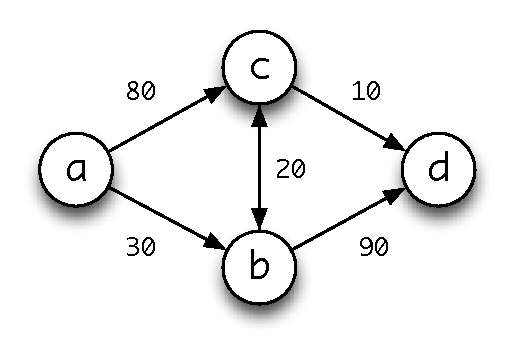
\includegraphics[width=0.2\textwidth]{eps/flight-costs}
  \vspace{-3mm}
  \caption{Costs between cities in the flight example}
  \label{fig:costs}
\end{figure}
\vspace*{-0.2cm}

\begin{lstlisting}[label=seller-cc,caption=Ticket seller's agent]
enum { N = 7 };
int t[N][3] =
{ { 2,3,10 },{ 0,1,30 },{ 1,2,20 },{ 2,1,20 },
  { 0,2,80 },{ 1,3,90 },{ 2,3,10 } };
int main() {
  for (int i = 0; i < N; i++)
    out("from_%d=1,to_%d=1,price=%d",
        t[i][0], t[i][1], t[i][2]);
  return 0;
}
\end{lstlisting}
\vspace*{-0.5cm}

\begin{lstlisting}[label=buyer-cc,caption=Ticket buyer's agent]
enum { N = 4 };
void wait_for_ticket(func_param p) {
  flt &d = *((flt *) p);
  char *str =
    in("from_%d=1 & to_%d=1 & price<=%d",
        d.from, d.next, d.cash);
  Ticket t = parse_ticket(str);
  fly(d.next, d.to, d.cash - t.price);
  cm();
}
void fly(int from, int to, int cash) {
  flt_info    flt[N];
  func_ptr    choices[N];
  func_param  params[N];
  if (from == to) return;
  visited[from] = true;
  vector<int> next = unvisited_neighbors();
  for (size_t i = 0; i < next.size(); i++) {
    flt[i] = flt_info(from, next[i], to, cash);
    choices[i] = wait_for_ticket;
    params[i] = (func_param) &(flt[i]);
  }
  gcc(choices, params, next.size());
}
int main() { fly(0, 3, 100); return 0; }
\end{lstlisting}

Table \ref{result_bobjill} shows the result of the experiment. 
%Both examples are repeated for 9 times, and the best and the worst cases 
Both examples are repeated nine times, and the minimum and the maximum 
number of worlds given.  
We see that the number of worlds can be small even with speculation
and the increase is also limited.
% Both the number of worlds and the memory cost are 
% limited in a reasonable range. 
%Notice that total number of worlds obtain in the worst case run
Notice that we only obtained a maximum of 67 worlds,
which is much smaller than the theoretical bound
of $2^{20}$ worlds (10 pairs of Bob vs. Jill agents).
The \emph{response time} is the time for the coordination server 
to process the first GCC request. 
The \emph{turnaround time} is the time to execute an agent program from 
start to finish, i.e. when all processes forked by this program exit.
There is variation in times and number of worlds
because GCC requests may be delayed randomly, 
and there is non-determinism in the execution of the agent programs/processes.
% and the operating system schedules the agent programs nondeterministically. 
%However, the gap between the best case and the worst one is relatively large, 
% However, the gap between the minimum case and the maximum one is relatively large, 
%   which indicates the system performance is not stable enough. 
%For the worst case of maximum turnaround time in the Bob-Jill cases, 
For the maximum case of maximum turnaround time in the Bob-Jill cases, 
the higher latency is caused by the use of the opportunistic forking mechanism 
which delays requests according to the number of worlds. 
Thus, even when there is no more requests, 
delayed requests may still have to wait.
% FOR Comment (5) of APPLC'12 REVIEWER 1
The response times are not small enough because of the delays as well.
This is a tradeoff between usage of system resources versus latency.
% Delayed requests require few system resources, so for an open system this is 
%   not harmful because further requests can still be processed. 

\begin{table}
\begin{center}
\begin{tabular}{c|c||c|c|c|c}
  \hline
  \multicolumn{2}{c||}{}
    & \multicolumn{2}{c}{Bob-Jill cases} & \multicolumn{2}{|c}{Flight cases} \\
    \cline{3-6}
  \multicolumn{2}{c||}{}
%    & best & worst & best & worst \\
     & min & max & min & max \\
  \hline
  \multicolumn{2}{c||}{Max \# of worlds}
    & 11 & 67 & 11 & 53 \\
  \hline
  \multicolumn{2}{c||}{Max storage (MB)}
    & 40.6 & 53.5 & 17.8 & 89.8 \\
  \hline
%  \multirow{2}{*}{Response time}
    Response
    & max
    & 9.22 & 133.62 & 10.34 & 67.91 \\
  \cline{2-6}
    time (s)
    & avg.
    & 4.44 & 44.48 & 3.36 & 17.05 \\
  \hline
%  \multirow{2}{*}{Turnaround time}
    Turnaround
    & max
    & 9.23 & 1011.91 & 10.34 & 67.91 \\
  \cline{2-6}
    time (s)
    & avg.
    & 5.07 & 318.19 & 3.36 & 17.05 \\
  \hline
\end{tabular}
\end{center}
\vspace{-3mm}
\caption{Experiment statistics}
\label{result_bobjill}
\end{table}

%{\bf KZ: If out of space, can cut the conclusion}

\section{Conclusion}  % Section 5

We have presented a concrete system architecture 
  and associated implementation and optimizations for GCC. 
This paper shows that GCC can be practical and realistic.
We show how to program in GCC by using our
  runtime system and how the agent programs work. 
% as well as our runtime 
%  system in terms of programmability and performance. 
The use of C/C++ as a host language demonstrates that 
GCC is language independent and embeddable in
mainstream languages. 

%\appendix
%\section{Appendix Title}
%
%This is the text of the appendix, if you need one.
%
%\acks
%
%Acknowledgments, if needed.

% We recommend abbrvnat bibliography style.

\bibliographystyle{abbrvnat}

% The bibliography should be embedded for final submission.

\bibliography{ocp,gcc}
%\begin{thebibliography}{}
%\softraggedright
%\end{thebibliography}

\end{document}
